% HOW TO USE THIS TEMPLATE 
% Read this before you start work on formating your thesis using Latex.
% Latex is the easiest way to format a thesis according to the NITT Guidelines. Latex takes care off tables, figures, chapters, sections and subsections and basically everything you need to keep track off. It will auto populate entries into the table of contents which is pretty useful and time-saving.
% This template was prepared assuming zero prior knowledge of Latex.
% THIS TEMPLATE WAS MADE FOR USE BY BTECH STUDENTS AND FOLLOWS THE THESIS GUIDELINES FOR BTECH STUDENTS
% Wherever possible, I have included examples and notes on how to modify the document to suit your needs. If your new to Latex, I would recommend not diverging from the instructions as you may end up with buggy sections. 
%
% I'll be using the notation where my comments explaining usage will be followed by a section of the code where you will find{BLOCK LETTERS}.
% This indicates that you have to modify only what's inside the curly braces. 




\documentclass[a4paper,12pt,oneside]{book}
\usepackage[utf8]{inputenc}
\usepackage{amssymb} 
\usepackage{amsmath}
\usepackage{listings}
\usepackage{color}
\definecolor{codegreen}{rgb}{0,0.6,0}
\definecolor{codegray}{rgb}{0.5,0.5,0.5}
\definecolor{codepurple}{rgb}{0.58,0,0.82}
\definecolor{backcolour}{rgb}{0.95,0.95,0.92}
\lstdefinestyle{mystyle}{
    backgroundcolor=\color{backcolour},   
    commentstyle=\color{codegreen},
    keywordstyle=\color{magenta},
    numberstyle=\tiny\color{codegray},
    stringstyle=\color{codepurple},
    basicstyle=\footnotesize,
    breakatwhitespace=false,         
    breaklines=true,                 
    captionpos=b,                    
    keepspaces=true,                 
    numbers=left,                    
    numbersep=9pt,                  
    showspaces=false,                
    showstringspaces=false,
    showtabs=false,                  
    tabsize=2
}
\lstset{style=mystyle}
\usepackage{graphicx}
\usepackage{float}
\usepackage[export]{adjustbox}
\graphicspath{ {images/} }
\usepackage{times}
\usepackage{geometry}
\usepackage{setspace}
\usepackage{tocloft}
\usepackage{tabu}
\usepackage{fancyhdr}
\geometry{a4paper, tmargin=1in, rmargin=1in, bmargin=1in, lmargin=1.5in}
\usepackage{titlesec}
\usepackage[toc,page]{appendix}
\titleformat{\chapter}[display]
  {\normalfont\huge\bfseries\centering}
  {\chaptertitlename\ \thechapter}{20pt}{\Huge}
  
\renewcommand{\cftchapleader}{\cftdotfill{\cftdotsep}} % for chapters
\renewcommand\contentsname{\centerline{TABLE OF CONTENTS}}
\pagestyle{fancy}
\cfoot{\thepage}
\rhead{}
\lhead{}
\renewcommand{\headrulewidth}{0pt}
\renewcommand{\footrulewidth}{0pt}

\begin{document}
% Change the title below to your own title E.g. \title{MYPROJECTNAME}
\title{B.Tech Thesis Template}
\frontmatter
\addtocontents{toc}{\textbf{Title}\hfill\textbf{Page No.}\par}
\begin{titlepage}
\begin{center}
% Insert your project title where it says {PROJECT TITLE}
\fontsize{18pt}{1cm}\selectfont \textbf{PROJECT TITLE}

\vspace*{1.4cm}
\fontsize{14pt}{21pt}\selectfont A thesis submitted in partial fulfillment of the requirements for\\
the award of the degree of

\vspace*{0.8cm}
\fontsize{14pt}{1cm}\selectfont\textbf{B.Tech.} 

\vspace*{0.8cm}
% Insert your branch in block letters where it says BRANCH NAME
\textbf{in\\BRANCH NAME}

\vspace*{2.0cm}
By
% Insert your name here under Name 1 and Name 2 as well as your respective Roll Numbers.
% To insert another name add this before the } --> \\NAME 3 (ROLL NUMBER)
\textbf{NAME 1 (ROLL NUMBER)\\NAME 2 (ROLL NUMBER)}

\vspace*{2.0cm}
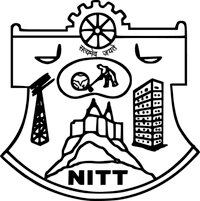
\includegraphics[width=1.25in]{NITT-Logo}

\vspace*{0.3cm}
% Insert Department Name where it says DEPARTMENT NAME
\fontsize{16pt}{16pt}\selectfont \textbf{DEPARTMENT OF \\DEPARTMENT NAME\\NATIONAL INSTITUTE OF TECHNOLOGY\\TIRUCHIRAPPALLI-620015}

\vspace*{0.5cm}
% You can change the month and year here
\textbf{MAY 2017}
\end{center}
\end{titlepage}
\thispagestyle{plain}
\begin{center}
\textbf{BONAFIDE CERTIFICATE}
\end{center}

\vspace{0.3cm}
% Enter the title of your project in the section where it says PROJECT NAME
\fontsize{12pt}{24pt}\selectfont This is to certify that the project titled \textbf{PROJECT NAME} is a bonafide record of the work done by
\vspace{1.0cm}

\begin{center}
% Insert your name here under Name 1 and Name 2 as well as your respective Roll Numbers.
% To insert another name add this before the } --> \\NAME 3 (ROLL NUMBER) 
\textbf{NAME 1 (ROLL NUMBER)\\NAME 2 (ROLL NUMBER)}
\end{center}

\vspace{1.0cm}
\noindent
% Insert the name of your branch where it says {BRANCH NAME}
\fontsize{12pt}{24pt}\selectfont in partial fulfillment of the requirements for the award of the degree of \textbf{Bachelor of Technology} in \textbf{BRANCH NAME} of the \textbf{NATIONAL INSTITUTE OF TECHNOLOGY, TIRUCHIRAPPALLI}, during the year 2016-2017.

\vspace{2.5cm}

\begin{tabu} to \textwidth { X[l] X[c] }

 \textbf{PROJECT GUIDE NAME} & \textbf{HOD NAME} \\
 Project Guide & Head of the Department

\end{tabu}

\vspace{2.0cm}
\noindent
\begin{tabular}{lc}
\fontsize{12pt}{24pt}\selectfont Project Viva-voce held on & \underline{\hspace{2in}}
\end{tabular}

\vspace{3.5cm}

\begin{tabu} to \textwidth { X[l] X[c] }

 \textbf{Internal Examiner} & \textbf{External Examiner}

\end{tabu}

\newpage
\addcontentsline{toc}{chapter}{ABSTRACT}
\thispagestyle{plain}
\begin{center}
\textbf{\textbf{\fontsize{16pt}{24pt}\selectfont ABSTRACT}}
\end{center}

\vspace{0.3cm}

% Start typing out your abstract after the \selectfont tag. And after your last line add a \\ if you require more spacing

\fontsize{12pt}{18pt}\selectfont Lorem ipsum dolor sit amet, consectetur adipiscing elit, sed do eiusmod tempor incididunt ut labore et dolore magna aliqua. Ut enim ad minim veniam, quis nostrud exercitation ullamco laboris nisi ut aliquip ex ea commodo consequat. Duis aute irure dolor in reprehenderit in voluptate velit esse cillum dolore eu fugiat nulla pariatur. Excepteur sint occaecat cupidatat non proident, sunt in culpa qui officia deserunt mollit anim id est laborum


% Enter keywords from abstract here
\textit{Keywords}: Lorem ipsum dolor sit amet

\newpage
\addcontentsline{toc}{chapter}{ACKNOWLEDGEMENT}
\thispagestyle{plain}
\begin{center}
\textbf{ACKNOWLEDGEMENT}
\end{center}

\vspace{0.3cm}
\noindent
\fontsize{12pt}{24pt}\selectfont We would like to thank the following people for their support and guidance without whom the completion of this project in fruition would not be possible.

\vspace{2.0cm}
\noindent
% Project guide name goes here
\fontsize{12pt}{24pt}\selectfont \textbf{PROJECT GUIDE NAME}, our project guide, for helping us and guiding us in the course of this project .\\

\vspace{1.0cm}

\noindent
% Head of Department and Department goes here under HEAD OF DEPARTMENT NAME AND DEPARTMENT NAME
\fontsize{12pt}{24pt}\selectfont \textbf{HEAD OF DEPARTMENT NAME}, the Head of the Department, Department of DEPARTMENT NAME.\\

\vspace{1.0cm}

\noindent
% Names of the Project Review Committee goes here (extra, but helps in buttering the review committee :p )
\fontsize{12pt}{24pt}\selectfont Our internal reviewers, \textbf{REVIEWER NAME 1} , \textbf{REVIEWER NAME 2} , \textbf{REVIEWER NAME 3} for their insight and advice provided during the review sessions. \\

\vspace{1.0cm}

\noindent
\fontsize{12pt}{24pt}\selectfont We would also like to thank our individual parents and friends for their constant support.\\

\newpage
\addcontentsline{toc}{chapter}{TABLE OF CONTENTS}
\tableofcontents
\newpage
\addcontentsline{toc}{chapter}{LIST OF TABLES}
\listoftables
\newpage
\addcontentsline{toc}{chapter}{LIST OF FIGURES}
\listoffigures
 
\mainmatter
% Create chapters by first adding a new .tex file with your chapter name. E.g. <ChapterFileName>.tex
% Insert your chapters here in the format specified below
% \chapter{ChapterName}
% \input{ChapterFileName}
% This will ensure that your chapter will be added to the table of contents
\chapter{Introduction}
% After creating your chapters and their names in main, you can enter your sections and subsections and sub sub sections in each chapter page. The table of contents will auto-fill the sections and sub sections automatically.


\section{Section Title}
Lorem ipsum dolor sit amet, consectetur adipiscing elit, sed do eiusmod tempor incididunt ut labore et dolore magna aliqua. Ut enim ad minim veniam, quis nostrud exercitation ullamco laboris nisi ut aliquip ex ea commodo consequat. Duis aute irure dolor in reprehenderit in voluptate velit esse cillum dolore eu fugiat nulla pariatur. Excepteur sint occaecat cupidatat non proident, sunt in culpa qui officia deserunt mollit anim id est laborum

\subsection{Subsection Title}
Lorem ipsum dolor sit amet, consectetur adipiscing elit, sed do eiusmod tempor incididunt ut labore et dolore magna aliqua. Ut enim ad minim veniam, quis nostrud exercitation ullamco laboris nisi ut aliquip ex ea commodo consequat. Duis aute irure dolor in reprehenderit in voluptate velit esse cillum dolore eu fugiat nulla pariatur. Excepteur sint occaecat cupidatat non proident, sunt in culpa qui officia deserunt mollit anim id est laborum

% Example on how to cite articles from bibliography. Use the \cite command to cite after entering article details in bibliography
As metioned in the article by Akram et al. \cite{akram} and the article by Xi et al. \cite{5334925} we have ...

\subsubsection{Sub Sub Section Title}
Lorem ipsum dolor sit amet, consectetur adipiscing elit, sed do eiusmod tempor incididunt ut labore et dolore magna aliqua. Ut enim ad minim veniam, quis nostrud exercitation ullamco laboris nisi ut aliquip ex ea commodo consequat. Duis aute irure dolor in reprehenderit in voluptate velit esse cillum dolore eu fugiat nulla pariatur. Excepteur sint occaecat cupidatat non proident, sunt in culpa qui officia deserunt mollit anim id est laborum
\chapter{Review Of Literature}
% This is an example on how to add pictures to Latex. The first example will cover using an image as free floating position (i.e. The positioning of the image is decided on where it will fit with the least wastage of space)
% By convention all image files should be added to a separate image folder. It is just easier to organize the project files that way.
\section{An Example On How To Add Pictures}
Lorem ipsum dolor sit amet, consectetur adipiscing elit, sed do eiusmod tempor incididunt ut labore et dolore magna aliqua. Ut enim ad minim veniam, quis nostrud exercitation ullamco laboris nisi ut aliquip ex ea commodo consequat. Duis aute irure dolor in reprehenderit in voluptate velit esse cillum dolore eu fugiat nulla pariatur. Excepteur sint occaecat cupidatat non proident, sunt in culpa qui officia deserunt mollit anim id est laborum

Example of using a label to refer to a Figure \ref{fig:NodeMCU}

% Example of free floating image
\begin{figure}
    \centering
    % Playing around with the [width=.8] value will resize your image according to its width. It will scale appropriately. The name of the image file goes under the {NodeMCU}
    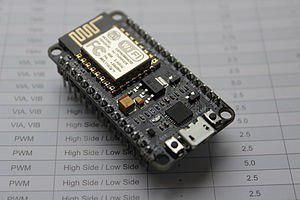
\includegraphics[width=.8\textwidth,center]{NodeMCU}
    \caption{NodeMCU Chip Diagram}
    % The label is useful when you want to refer to your image from text but you don't know what figure number it is.
    \label{fig:NodeMCU}
\end{figure}


\section{Fixed Image}Lorem ipsum dolor sit amet, consectetur adipiscing elit, sed do eiusmod tempor incididunt ut labore et dolore magna aliqua. Ut enim ad minim veniam, quis nostrud exercitation ullamco laboris nisi ut aliquip ex ea commodo consequat. Duis aute irure dolor in reprehenderit in voluptate velit esse cillum dolore eu fugiat nulla pariatur. Excepteur sint occaecat cupidatat non proident, sunt in culpa qui officia deserunt mollit anim id est laborum 

% To fix images to a certain section or sub section, do as follows

I want my image fixed here
 % The [H] after {figure} fixes the positioning of images.
\begin{figure}[H]
    \centering
    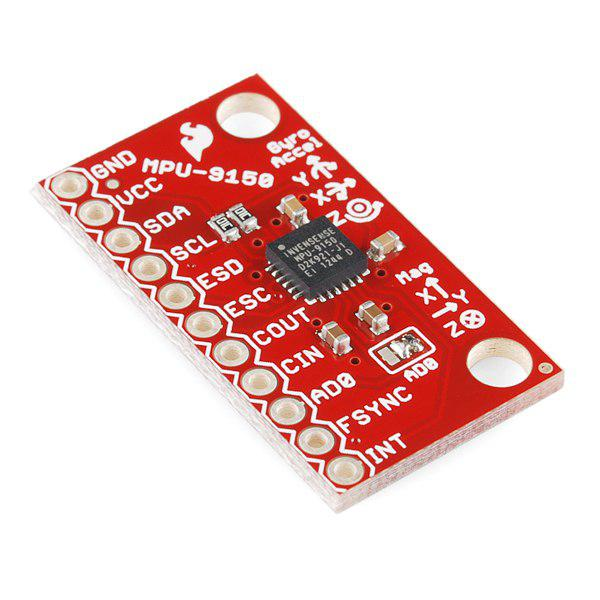
\includegraphics[width=.8\textwidth,center]{Inert}
    \caption{Inertial Measurement Unit}
    \label{fig:IMU}
\end{figure}

\section{Example on Table Usage}

Lorem ipsum dolor sit amet, consectetur adipiscing elit, sed do eiusmod tempor incididunt ut labore et dolore magna aliqua. Ut enim ad minim veniam, quis nostrud exercitation ullamco laboris nisi ut aliquip ex ea commodo consequat. Duis aute irure dolor in reprehenderit in voluptate velit esse cillum dolore eu fugiat nulla pariatur. Excepteur sint occaecat cupidatat non proident, sunt in culpa qui officia deserunt mollit anim id est laborum
\\
% To refer to the table use the same \ref{table:Spec}
To refer to the table use the same \ref{table:Spec}

\begin{table}[h!]
\centering
% To add another column in the table add another c in ||c c|| such that you get ||c c c|| for a three column table
\begin{tabular}{||c c||} 
 \hline
 %Every row entry is separated by a &. This is for Column titles.
 MPU 9150 Inertial Measurement Unit & NodeMCU Processor \\ [0.5ex] 
 \hline\hline
 % Data rows go here
 Acceleration Range: 2G & Dual-Core 80 Mhz Processor \\ 
 Gyroscope Range: 250 degrees/second  & 4MB Flash Memory \\
 Magnetometer Range: 1200 micro Teslas & 802.11 b/g/n connectivity \\
 Communication Protocol: I2C & \\[1ex] 
 \hline
\end{tabular}
\caption{Sensor Specifications}
\label{table:Spec}
\end{table}


\newpage
% The bibliography goes under a separate .bib file. To quote articles, just fill the appropriate headings in the bibliography file. 
\addcontentsline{toc}{chapter}{References}
\bibliographystyle{unsrt}
\bibliography{reference}

\begin{appendices}
\addtocontents{toc}{\protect\setcounter{tocdepth}{0}}
% Appendix chapters go here. Note that appendix will not show sections or subsections as the main chapters above in the table of contents. Also chapter numbering will be alphabetic e.g. (A,B,C etc) The example on the appendix also shows how to add programming code to a thesis.
  \chapter{Code Attachments}
  \section{Lorem Ipsum}
Lorem ipsum dolor sit amet, consectetur adipiscing elit, sed do eiusmod tempor incididunt ut labore et dolore magna aliqua. Ut enim ad minim veniam, quis nostrud exercitation ullamco laboris nisi ut aliquip ex ea commodo consequat. Duis aute irure dolor in reprehenderit in voluptate velit esse cillum dolore eu fugiat nulla pariatur. Excepteur sint occaecat cupidatat non proident, sunt in culpa qui officia deserunt mollit anim id est laborum 

% The following example is for writing Code in a Latex Environment
% The listings package is used to make code appear in an ordered and indented manner. Note that every code section begins with a \begin{lstlisting}[Language=Python]. Change language to the programming language of your choice and the syntax highlighting will change accordingly
\begin{lstlisting}[language=Python]
def get_parameters(data, chunk_size=410):
	#Store the activity label to add later
	activity = data['Activity']
    '''
    Define a dictionary of functions. Sets of readings will be aggregated as per these functions
    '''
	func_dict = {
		'min': np.min,
		'max': np.max,
		'diff': lambda x: np.max(x) - np.min(x),
		'std': np.std,
		'iqr': stats.iqr,
		'rms': lambda x: np.sqrt(np.mean(np.square(x))),
		'mad': lambda x: x.mad(),
		'mediad': mediad
	}
	aggregations = {
		'X': func_dict,
		'Y': func_dict,
		'Z': func_dict
	}
	data_groups = []
    '''
    Transform the dataset into rolling windows of 410 readings each and store them in a Pandas data group.
    '''
	for i in range(int(data.shape[0]/(chunk_size/2)) - 1):
		temp = data.iloc[int(i*(chunk_size/2)):int((i+2)*(chunk_size/2))]
		temp['k'] = i
		data_groups.append(temp)
	data_groups = pd.concat(data_groups).groupby('k', as_index=False)
    #Run the aggregations on all data groups
	stats_data = data_groups.agg(aggregations)
	stats_data.columns = [''.join(col).strip() for col in stats_data.columns.values]
	activity = activity.reset_index(drop=True)
    #Add activity label
	stats_data = pd.concat([stats_data, activity[:len(stats_data)]], axis=1)
	del stats_data['k']
	return stats_data
\end{lstlisting}


\end{appendices}



\end{document}
